\chapter{Results}\label{ch:results-evaluation-conclusion}

\section{Summary}\label{sec:results}

\subsection{Smart contract}\label{subsec:res-smart-contract}

\begin{figure}[H]
    \centering
    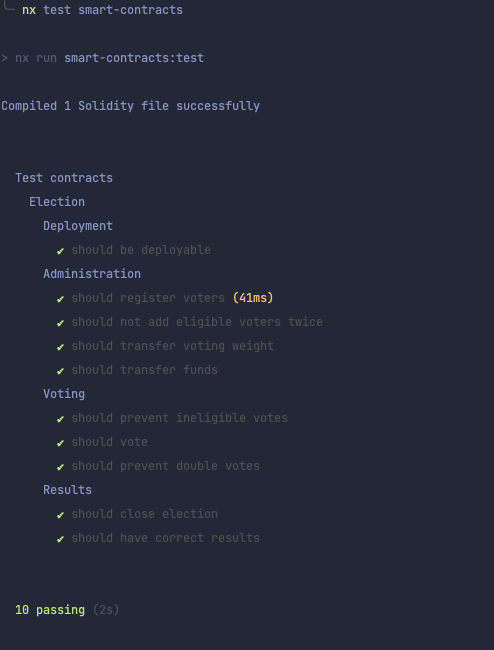
\includegraphics[scale=0.7]{boehm-testing-contract}
    \caption[Smart contract test results]{Smart contract test results. Screenshot taken by author}
    \label{fig:smart-contract-test-results}
\end{figure}

We tested the Solidity code of our \gls{SmartContract} using a JavaScript test suite and the contract's \gls{ABI} (see~\cref{subsec:unit-tests,subsec:testing-the-contract}).
The contract's functions are called in the order they would be called in during an election.
As shown in~\cref{fig:smart-contract-test-results}, the contract's bytecode is deployable to any network that supports Solidity.
Furthermore, all its functions made the expected changes to its internal state and rejected invalid transactions.
Thus, we could show that the contract would ensure a secure election process when deployed (see \cref{subsec:qualitative-objectives,sec:voting-systems}).

\subsection{End-to-end tests}\label{subsec:res-end-to-end-tests}

As seen in~\cref{fig:apx-e2e-tests-1}, we tested the initialization and services of the server's auth module.
In order to prevent users from having multiple accounts, we check entered \glsplural{SSN} and email addresses against our database.
Ultimately, governments would probably implement an \gls{API} in their backend services to validate voters' \glsplural{SSN}.
Regardless of the implementation, our \gls{E2E} tests showed that validating a voter's identity by his \gls{SSN} is a secure way for governments to ensure unique accounts, which is one aspect of providing a secure electronic voting system (see \cref{subsec:qualitative-objectives,sec:voting-systems}).

\begin{figure}[H]
    \centering
    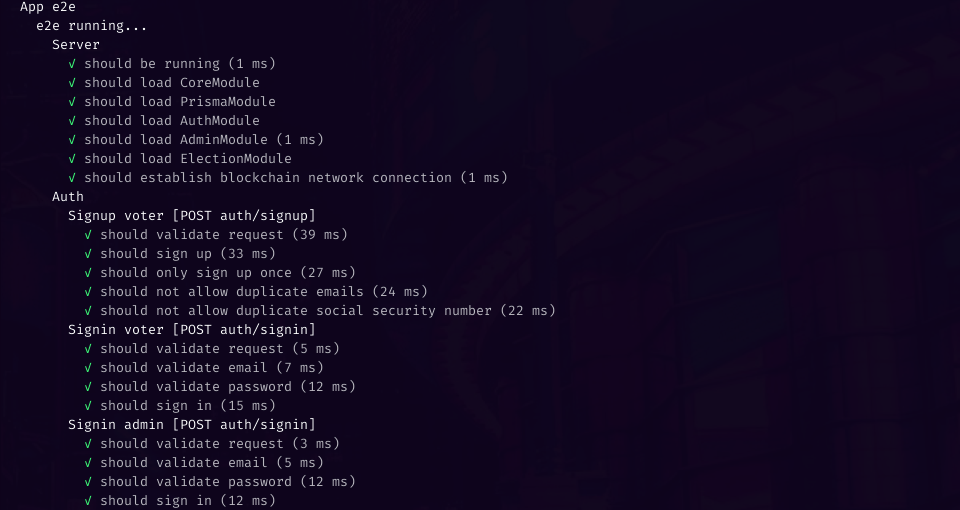
\includegraphics[width=\textwidth-50px]{boehm-e2e-tests1}
    \caption[Server E2E test results of initialization and auth module]{Server E2E test results of initialization and auth module. Screenshot taken by author}
    \label{fig:apx-e2e-tests-1}
\end{figure}

Another aspect is the protection of routes.
Since we aimed to create a system that enables election officials to create and deploy decentralized elections without prior experience developing \glsplural{SmartContract} (see \cref{subsec:quantitative-objectives}), we implemented access control using \glsplural{JWT} (see \cref{subsec:security}).
Consequently, we also tested whether the implemented protection works (see \cref{fig:apx-e2e-tests-2}), showing that \glsplural{JWT} can secure access to server routes.

\begin{figure}[H]
    \centering
    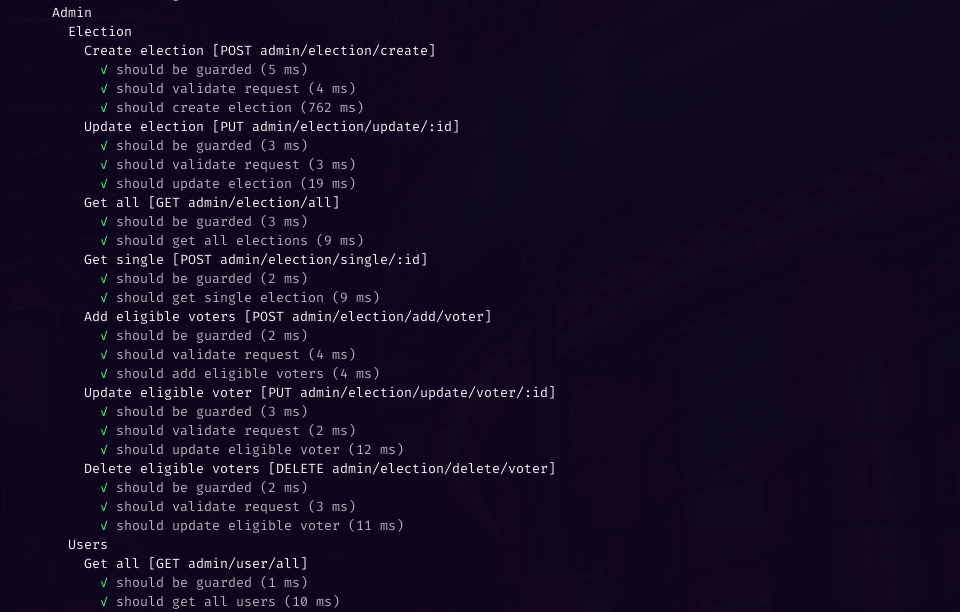
\includegraphics[width=\textwidth-50px]{boehm-e2e-tests2}
    \caption[Server E2E test results of admin module]{Server E2E test results of admin module. Screenshot taken by author}
    \label{fig:apx-e2e-tests-2}
\end{figure}

\begin{figure}[H]
    \centering
    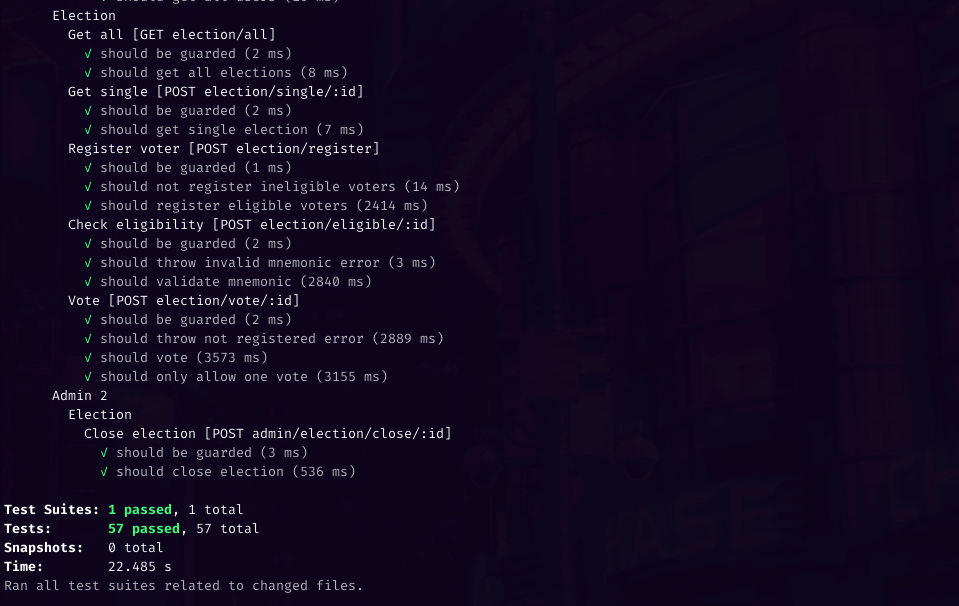
\includegraphics[width=\textwidth-50px]{boehm-e2e-tests3}
    \caption[Server E2E test results of election module]{Server E2E test results of election module. Screenshot taken by author}
    \label{fig:apx-e2e-tests-3}
\end{figure}

The tests were also designed to simulate an \gls{E2E} voting process.
Our \gls{E2E} tests proved that users could not register for an election they are not eligible to vote in (see \cref{fig:apx-e2e-tests-3}).
Also, once they had registered for an election, they could not submit a vote without possessing a registered \gls{PK}-\gls{PBK} key pair since the deployed \gls{SmartContract} only allows transactions from addresses registered in its internal state.
In conclusion, the election's integrity (see \cref{subsec:qualitative-objectives,sec:voting-systems}) is ensured due to the immutability of data stored on \gls{Blockchain} networks (see \cref{sec:blockchain}).

\subsection{Scalability test}\label{subsec:res-scalability-test}

As mentioned in \cref{subsec:quantitative-objectives,sec:voting-systems}, scalability is a crucial feature of any voting system employed in national elections.
In this context, scalability refers to two aspects: processing time, i.e., how much time the system needs to process a number of voters, and the processing cost.
Accordingly, as mentioned in \cref{subsec:scalability-tests}, we wrote additional tests that generated high network traffic by simulating a statistically significant number of voters.

\subsubsection{Consecutive votes}\label{subsubsec:res-consecutive-votes}

\begin{figure}[h]
    \centering
    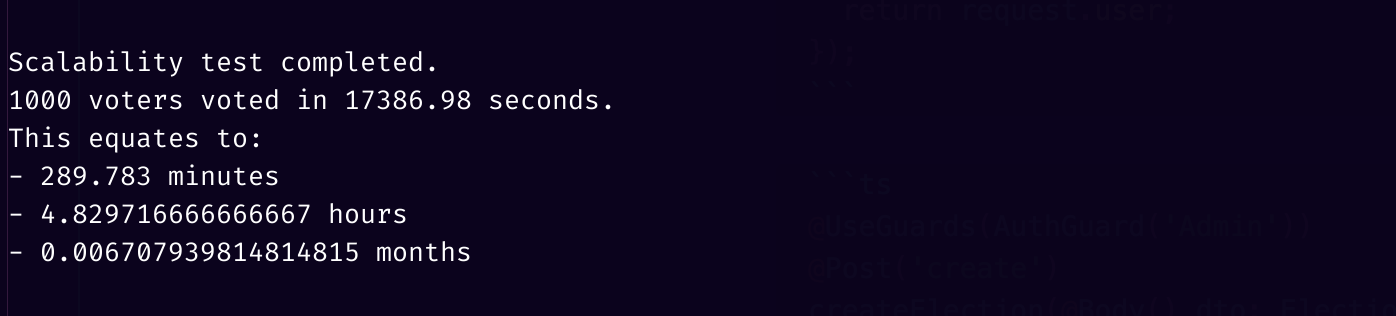
\includegraphics[width=\textwidth]{boehm-scalability-test-result}
    \caption[Scalability test result]{Scalability test result. Screenshot taken by author}
    \label{fig:scalability-test-result}
\end{figure}

Simulating consecutive registrations and votes in an election resulted in a processing time of 17,386.98 seconds or 4.83h hours for 1,000 voters (see \cref{fig:scalability-test-result}) with 1\% of votes not being processed with the first request.
Consequently, it would take 13,4158.80 months to process a national election with 20,000,000 eligible online voters consecutively, which is not feasible for an election.
Ultimately, this means that any system employed in national elections must be capable of processing votes concurrently.

\subsubsection{Concurrent votes}\label{subsubsec:res-concurrent-votes}

Unfortunately, the scalability test recorded a 100\% failure rate in concurrent mode.
This could be attributed to a design flaw in our backend services that made the system unable to commit concurrent transactions to the \gls{Blockchain} due to transactions sharing the same transaction nonce.
As a result, the \gls{Blockchain} network registered those transactions as a single transaction, with the latter transactions trying to override the former ones.

\subsection{Transaction analysis}\label{subsec:res-transaction-analysis}

The scalability test generated transactions on the \gls{Blockchain}, enabling us to evaluate voter anonymity, auditability, and scalability in the context of operational costs by using a \gls{BlockExplorer} (see \cref{subsec:qualitative-objectives,sec:voting-systems}).
The transaction history of the \gls{SmartContract} we used for testing can be independently verified on \href{https://mumbai.polygonscan.com/address/0x626aec8b9220bee641bc4098fa73f8cc55e50a8f}{Polygonscan}.

\subsubsection{Anonymity}

\begin{figure}[h]
    \centering
    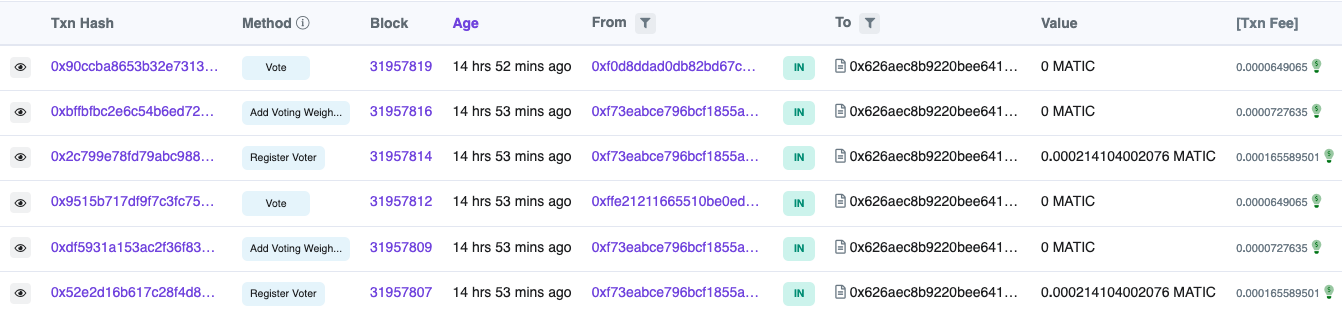
\includegraphics[width=\textwidth]{boehm-transaction-analysis}
    \caption[Smart contract transaction history]{Smart contract transaction history on \href{https://mumbai.polygonscan.com/address/0x626aec8b9220bee641bc4098fa73f8cc55e50a8f}{Polygonscan}. Screenshot taken by author}
    \label{fig:transaction-analysis}
\end{figure}

As shown in~\cref{fig:transaction-analysis}, even though all transactions are publicly visible through the use of a \gls{BlockExplorer}, no identifying information about voters is committed to the \gls{Blockchain} as all transactions are made by our system using voters' wallets.
Hence, the only information the public would have on an individual voter is his \gls{PBK} and the approximate transaction time.

\subsubsection{Auditability}

\begin{figure}[h]
    \centering
    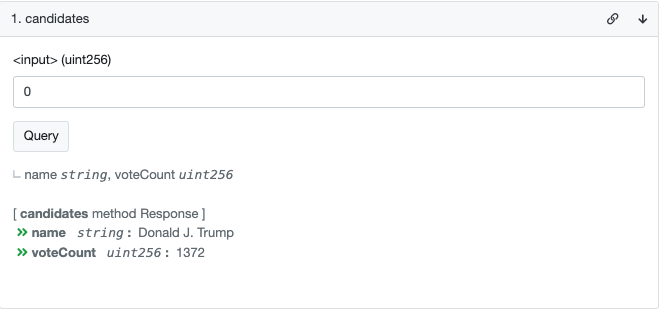
\includegraphics[width=\textwidth]{boehm-audit}
    \caption[Smart contract audit]{Smart contract audit on \href{https://mumbai.polygonscan.com/address/0x626aec8b9220bee641bc4098fa73f8cc55e50a8f}{Polygonscan}. Screenshot taken by author}
    \label{fig:audit}
\end{figure}

The public can independently audit the election in precisely the same manner, using a \gls{BlockExplorer} to analyze all transactions on the election’s \gls{SmartContract} and to call the contract’s functions to evaluate its internal state of the election result (see \cref{fig:audit}).

\subsubsection{Transaction costs}\label{subsubsec:res-transaction-costs}

\begin{figure}[h]
    \begin{subfigure}[b]{0.5\textwidth}
        \centering
        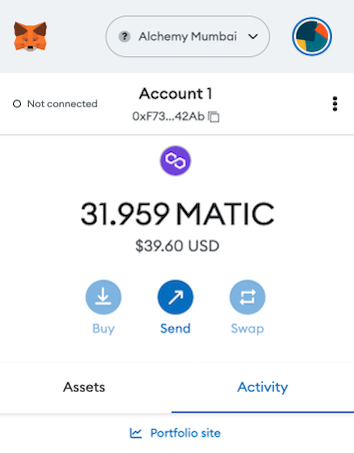
\includegraphics[width=\textwidth]{boehm-balance1}
        \caption{Balance before scalability test}
        \label{fig:balance-before}
    \end{subfigure}
    \begin{subfigure}[b]{0.5\textwidth}
        \centering
        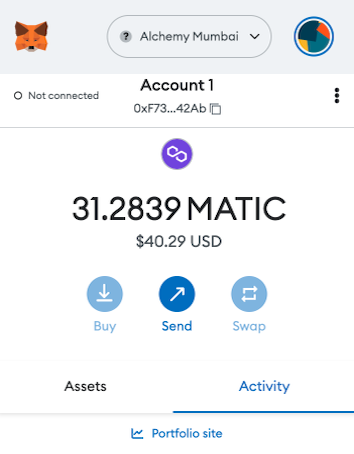
\includegraphics[width=\textwidth]{boehm-balance2}
        \caption{Balance after scalability test}
        \label{fig:balance-after}
    \end{subfigure}
    \caption{Transaction costs. Screenshots taken by author.}
    \label{fig:transaction-costs}
\end{figure}

As seen in \cref{fig:transaction-analysis}, the \gls{E2E} process for a single vote in an election generates three transactions on the corresponding smart contract, each costing approximately 0.0000649 to 0.000166 MATIC in fees equalling \$0.000084 to \$0.000214 at the time of this writing.
Additionally, a small amount of MATIC, calculated based on average network fees at the time of the transaction, is transferred to voters' wallets.
Accordingly, as shown in \cref{fig:transaction-costs}, the administrating wallet's balance before running the scalability test was 31.959 MATIC (see \cref{fig:balance-before}) and 31.2839 MATIC (see \cref{fig:balance-after}) after having processed 1000 voters.
Innately, MATIC prices fluctuated while running the tests causing the lower balance in \cref{fig:balance-after} to have a higher exchange value when calculated in US dollars.
Regardless, at the time of this writing, the difference between both balances equaled \$0.87.
Hence, we can safely conclude that our system is scalable in terms of operational costs.
In fact, it is much cheaper to operate than traditional analogous or centralized e-voting systems which cost around \$10/voter~\autocite{mohr_how_nodate}.


\subsection{Quantitative Objectives}\label{subsec:res-quantitaive-objectives}

We aimed to create user interfaces that would take a voter through the \gls{E2E} process of voting in an election while simultaneously providing authorized election officials to create an election without prior experience in \gls{SmartContract} programming (see \cref{subsec:quantitative-objectives}).
As seen in \cref{subsec:pages,ch:video-of-e2e-election-process}, we achieved all of those objectives.
The client application of our voting system enables officials to create new elections by filling out a form and registered users to visually identify an election they wish to vote in, register for the selected election and vote for a candidate.

\section{Evaluation}\label{sec:evalutaion}

\subsection{Personal scrum}\label{subsec:res-personal-scrum}

Our adherence to scrum methods (see \cref{subsec:personal-scrum}) kept the project on track during planning and development and significantly improved our ability to track and resolve issues.
However, the personal scrum method is missing one of the most crucial incremental parts, code reviews.
Instead, we relied on \gls{E2E} testing and regular functional testing of the developed web client to substitute for this.
Although this method proved effective for finding and fixing several bugs, detailed code reviews would have been a preferable addition to the evaluation process of this project.

\subsection{Monorepo}\label{subsec:monorepo}

We used nx (see \cref{subsec:nx,subsec:creating-a-monorepo-using-nx}) to develop all project applications in a single repository.
This decision significantly improved development times since we could streamline and simplify project dependencies.
Nevertheless, monorepos also come with challenges.
For example, we did not implement continuous integration for this project which, in our experience, is a more demanding task in a monorepo.

\section{Conclusion}\label{sec:conclusion}

We successfully developed an electronic voting system prototype that processes votes decentrally on any blockchain network whose virtual machine can execute Solidity code.
In summary, elections conducted with our system were highly transparent due to the ease of auditing transactions and election results using a \gls{BlockExplorer} (see \cref{subsec:res-transaction-analysis}).
Additionally, we measured high levels of security and anonymity as well as low operational costs (see \cref{subsec:res-smart-contract,subsec:res-end-to-end-tests,subsec:res-transaction-analysis}).

Even so, due to the complexity of the technology, weighing certain accessibility features against security and anonymity proved to be very challenging.
Furthermore, scalability in terms of transaction speed remains to be one of the most significant hurdles despite meaningful innovations in this area in recent years.
The current state of the technology is that, even in theory, no protocol can process a high enough number of votes for a national election which would entail millions of transactions in a single day.

To test our system, we chose Polygon as we concluded from our research that the network, while still not being fast enough in theory, could deliver the highest number of \gls{TPS}.
However, as discussed in \cref{subsec:res-scalability-test}, a design flaw in our backend services made it impossible for our application to process concurrent votes.
Accordingly, further research should consider a server design that handles concurrent requests and transactions to the chosen network.
In our estimation, this could be achieved by building a queuing system into the server’s service that assigns requests to several administrative wallets, which then process transactions by iterating on a nonce.
Alternatively, possibilities to make all transactions on the client side could be explored, which would alleviate the problem while improving decentralization and thereby the system’s security.
Although, it should be noted that during our research, complete decentralization proved challenging to achieve without sacrificing accessibility to a certain degree.

Overall, taking into account areas of concern such as scalability and potential unforeseen security risks of decentralized voting systems, we recommend further research into the practical development of such systems with the aim of rolling out local pilot programs.